\documentclass{article} % For LaTeX2e
\usepackage{hyperref}
\usepackage{url}
\usepackage{amsmath} % Required for some math elements 
\usepackage{graphicx} % Required for the inclusion of images
\usepackage{natbib} % Required to change bibliography style to APA


\title{COMP 408/ELEC 408 Project Proposal:\\ NDVI of Satellite Images using CUDA Thrust}


\author{
Ahmet Uysal - 60780\\
\href{mailto:auysal16@ku.edu.tr}{\texttt{auysal16@ku.edu.tr}}\\
 \\
Halil Eralp Ko\c{c}a\c{s} -53618\\
\href{mailto:hkocas15@ku.edu.tr}{\texttt{hkocas15@ku.edu.tr}}
}

\begin{document}

\maketitle

\begin{abstract}
Applying NDVI algorithms to satellite images can give helpful insights about the quality of the crops, change over time and drought. However, since the size of the images are too large, classical implementations requires too much time and processing power. Processing power of the Graphics Processing Unit (GPU) can be used to implement NDVI algorithms faster and cheaper. In this project, we will use Thrust library of Nvidia CUDA platform to apply NDVI algorithm to images acquired from Sentinel-2 satellite, using GPU similarly to the article of Alvarez et al.\cite{ndvi-thrust}. 
\end{abstract}

\section{Introduction}

\subsection{What is NVDI?}
NDVI (Normalized Difference Vegetation Index) detects the portion of vegetation by measuring the difference between near-infrared and red light. Vegetation reflects the near-infrared light; however, it absorbs red light. NDVI’s range is always from -1 to 1. For instance, when the NDVI is close to -1, it is highly possible you are looking for water area. On the other hand, when it is close to +1, you are most probably looking for densely green area. Further, when the NDVI is around 0, you are probably looking for urbanized area. The NDVI can be calculated by the following formula:

\begin{equation*}
NDVI = \frac{NIR - Red}{NIR + Red}
\end{equation*}

Healthy vegetation reflects more NIR (near infra-red) and green light, on the other hand, it absorbs more red and blue lights. 

\newpage

\subsection{Sample Results}

The images are taken from GISGeography website\cite{gisgeography_2018}

\begin{figure}[!htb]
\centering
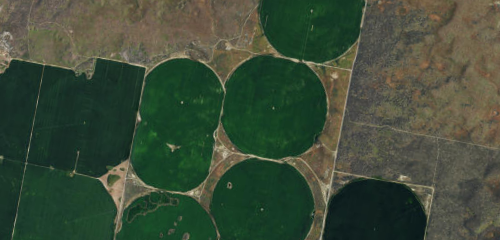
\includegraphics[width=0.7\textwidth]{ndvi-normal.png}
\caption{Original satellite image.}
\end{figure}

\begin{figure}[!htb]
\centering
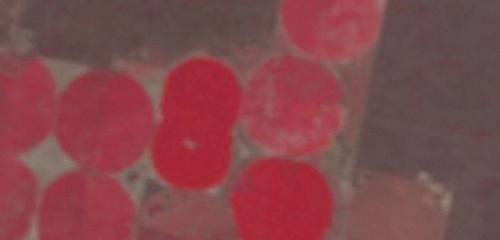
\includegraphics[width=0.7\textwidth]{ndvi-nir.png}
\caption{Near Infrared (NIR) band applied image.}
\end{figure}

\begin{figure}[!htb]
\centering
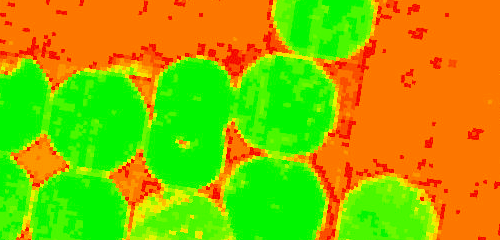
\includegraphics[width=0.7\textwidth]{ndvi-ndvi.png}
\caption{Normalized Difference Vegatation Index (NDVI) result of image.}
\end{figure}

\newpage

\section{Current Progress}	

We investigated image sources and found that ESA shares Sentinel-2 satellite images. We created an image set using their platform.

%\section{Baseline or Initial Experiments}
%
%
%\section{Proof of Concept}
%Now you are ready to begin the meat of your project, but you know that development will take some time. To avoid the nightmare scenario in which you spend most of your time working on an inherently flawed approach, you will need to find a toy problem or sub-problem to validate your approach(es) well before the deadline. It is also critical that the problem be simple enough such that the outcome is interpretable and the following questions (and others) can be answered:
%
%\textit{Is it failing because of a bug in our program or because of an issue with out approach? Why isn't this strategy performing as well as we hoped? Is there a reasonable adjustment we can make to do better? Do we need to pivot?}
%
%In this section, describe such a suitable problem and how you will evaluate the results. If applicable, list the different approaches you will be evaluating on this problem (e.g. you have two candidate algorithms for your project task).
%
%\section{Final Experiments}
%
%After you successfully evaluate your approach(es) on a smaller problem, it's now showtime. How will you move beyond this small problem and adapt your technique for the ultimate challenge? What experiments do you plan to run? This section can be less developed and speak in terms of the results of earlier experiments. You should also more thoroughly describe the setup of these final experiments and how it relates to your end goal.

\section{Final Goals}

At the end of the semester we want to be able to give detailed reports about percentage of vegetation, drought, seasonal changes of the vegetation using different images. Using periodically taken satellite images, we can track the development of agricultural crops using NDVI. This project can be integrated into a mobile application that aims to help farmers track their field and their crops. 


\begin{itemize}
\item By the end of the semester we want to successfully analyze the satellite images using NDVI on GPU.
\item In later stages, we want to automatize the process of downloading satellite images using Copernicus APIs and be able to track one location continuously.
\item The final goal is the integration of this project into a mobile application where farmers can get periodical reports about their field and crops.
\item For further progress, machine learning models can be added to project to allow kind-specific crop analysis based on what farmer has on his/her field.
\end{itemize}

\section{Data \& Technical Requirements}

Copernicus Services Data Hub is used to acquire Sentinel-2 satellite images. CUDA Thrust C++ Library will be used to implement NDVI on GPU. We are planning to run the project on our computer with \href{https://www.geforce.com/hardware/desktop-gpus/geforce-gtx-1060/specifications}{Nvidia GeForce GTX 1060} graphics card. However, cloud GPU providers such as Google Colab can be used if it is needed. For the later usage and processing of generated NDVI images, OpenCV library will be used.


% You should cite all sources mentioned in this proposal in the file 11785_project.bib
% If you don't wish to cite some of your sources inline (e.g. in the Related Work section) using \cite{}, just you nocite to add
% them to the references section at the end of your proposal like so.
%\nocite{Bengio+chapter2007}
%\nocite{Hinton06}

\bibliography{references}
\bibliographystyle{abbrv}


%\bibliographystyle{apacite}
%\bibliography{citation-ndvi-thrust}
%\bibliographystyle{citation-ndvi-thrust}

\end{document}
